\documentclass[main.tex]{subfiles}
\begin{document}

\chapter{The Triplets...}

%\textbf{NL:  This chapter seems to assume a priori that the reader will be familiar with orbital dynamics and the two-body problem. Need to go through it carefully, and be sure the concepts are introduced in the right order.  But this chapter will mostly be about orbital dynamics, and the two- and three-body problems.}

%THIS CHAPTER DESCRIBES THE OUTER TRIPLE EXCITING LK OSCILLATIONS IN THE INNTER TWO BINARY COMPONENTS, EVENTUALLY CAUSING THEM TO MERGE IN A HORRIFIC AND GORY FINAL FATE.  THE NEW EMERGING SIBLING, WHILE MUCH MORE MASSIVE, IS SWEET AND KIND, AND TWEEDLEDOH IS VERY HAPPY TO MEET HIS NEW SISTER TWEEDLEDAH.
 
%Alone at last ...well, depending on how you looked at it.  
\par \nar Now gravitationally unbound from their siblings, \rmtaygete, \rmalcyone~ and \rmcelaeno~ find themselves drifting off in to the vastness of empty space$^{\textcolor{red}{\ref{boxchap3:dynI}},\textcolor{blue}{\ref{boxchap3:dynII}}}$.  

\section{Two's Company, Three's a Crowd}

\par \nar Three siblings alone at last.  Well, two twins and a target: the inner twins continued to gossip rudely about their outer, omni-present sister.

\par \Taygete She's a little bulbous don't you think?

\par \Alcyone  Ha ha.  Yeah, you nailed it!

\par \Celaeno  I can \textit{still} hear you two.  And I am \textit{not} bulbous.  A little round perhaps, but never bulbous.  And I shine brighter than either one of you.  So take that!

\par \Alcyone You may shine brighter than each of us individually, but together \textit{we} outshine \textit{you}.  

\par \Taygete Yeah!  Take \textit{that}!

\par \nar \rmcelaeno~ lets out a long, exasperated sigh.

\par \Celaeno My sisters, I really don't want to fight with you.  First, we're sisters from the same Mother.  Second, we're pretty much stuck together in this configuration for the next several hundred million years.  So we had might as well make the most of it.

\par \Taygete \textit{Fat} chance, you bulbous sphere!

\par \Alcyone Ah ha, another good one, sister!

\par \Celaeno Well, fine.  I guess I'll take a nap then.  Better than listening to the two of you...

\section{The Demise of \rmtaygete~ and \rmalcyone}

\par \nar After some time, \rmcelaeno~ awoke from a peaceful slumber.  

\par \Celaeno Yaaaaawn... What a great nap. 
% \rmtaygete~ and \rmalcyone?

\par \nar \rmcelaeno~ turned her gaze toward her sisters, but was horrified by what she saw.  Her sisters' relative distance\footnote{In other words, the distance separating their respective centers of mass.} had changed over the course of their slumber.  It had gone \textit{down}, in fact.  They were now orbiting their common center of mass closer than ever before.  What's more, it seemed to \rmcelaeno~ that the relative angle of inclination between the inner orbital plane formed by her sisters's orbital plane and her own outer orbital plane had changed$^{\textcolor{red}{\ref{boxchap3:incl}}}$.  They were now much more coplanar than before.

%\footnote{That is, all three stars orbiting within the same 2-D plane.}  In fact, currently, \rmcelaeno~ could only see \rmalcyone~ directly; presumably, \rmtaygete~ was behind \rmalcyone, her light being eclipsed by the foreground presence of her twin sister, along the line of sight separating her from \rmcelaeno.

\par \nar  In fact, currently, \rmcelaeno~ could only see \rmalcyone~ directly; presumably, \rmtaygete~ was behind \rmalcyone, her light being eclipsed by the foreground presence of her twin sister, along the line of sight separating her from \rmcelaeno.

\par \nar Rather crucially, \rmtaygete~ and \rmalcyone~ now shared a much more eccentric orbit than before$^{\textcolor{red}{\ref{boxchap3:ecc}}}$.

\par \nar In particular, they now swung out to larger relative distances with respect to their common center of mass; here, they sit patiently due to their much slower orbital velocities. 

\par \nar But, they eventually swing to much closer approaches than before, their surfaces almost touching at the point of closest approach$^{\textcolor{red}{\ref{boxchap3:periapo}},\textcolor{blue}{\ref{boxchap3:dynIII}},\textcolor{green}{\ref{boxchap3:dynIV}}}$.

\par \nar Each time they complete one orbital revolution, the two sisters drift a little bit closer to colliding directly with each.  On the whole, there was no mistaking the fact that their orbit was getting more compact...and fast$^{\textcolor{blue}{\ref{boxchap3:stab}}}$.

\par \nar After a particularly close periastron passage, \rmtaygete~ too began to notice the changes.

\par \Taygete  Whoa!  What the heck is going on?!  I almost just collided with \rmalcyone!

\par \Alcyone Uh yeah, no kidding!  That was a close call.  What the heck \textit{is} going on?!  Don't get so close to me the next time you pass back around, \rmtaygete~...

\par \Taygete It's not like I am doing it on purpose...

\par \Celaeno  Well, don't panic just yet.  We need to figure this out, since I can't very well run off to bring back help.

\par \Alcyone Useless to the bitter end...

\par \Celaeno Cram it.  

\par \Alcyone Wait... Cram what exactly?

\par \Celaeno Your mouth.  

\par \Alcyone With what?

\par \Celaeno Anything that prevents you from talking.  

\par \Alcyone You do realize we are floating in the emptiness of an infinite vacuum, right?  It's slim pickings I am afraid, at least in so far as cramming materials are concerned.

\par \Celaeno Right, fair enough.  The point is:  stop being a jerk.  And while you are doing that, I am going to try to figure out a way to save you.  I suspect that the shift toward more co-planar orbits is directly related to the increase in your orbital eccentricity.  If you think about it, these two things in combination should conserve total angular momentum, and might arise if the components of the inner orbit spend more or less time above or below the orbital plane of the outer orbit.\footnote{Sir Isaac Newton was among the first to consider the mutual gravitational interactions of a hierarchical triple star system.  He realized that, if the orbital plane of the inner compact binary is inclined relative to the outer orbit of the tertiary companion, then an asymmetry can arise where the components of the inner binary do not spend equal amounts of time above and below the orbital plane of the tertiary.  This provides a net torque on the inner binary, reducing its orbital inclination with respect to the outer tertiary orbital plane.  In order to conserve angular momentum, the eccentricity of the inner binary must increase, reaching a maximum when the orbital plane of the inner binary crosses that of the outer tertiary.  If the eccentricity gets to be sufficiently high, then the components of the inner binary can collide and merge.  For triples that do not undergo a collision in the inner binary, these oscillations in orbital inclination and eccentricity are nowadays called "Lidov-Kozai oscillations".} 

\textcolor{cyan}{NL:  I covered both of these in Chapter 2, but not really conservation laws.}
\begin{comment}
%\footnote{DEFINE ANGULAR MOMENTUM AND CONSERVATION THEREOF.}
\begin{tcolorbox}[sharp corners, colback=red!30, colframe=red!80!blue, title=Angular Momentum]
\par \textcolor{red}{DEFINE ANGULAR MOMENTUM.}. 
\end{tcolorbox}

%LEVELTWO:
\begin{tcolorbox}[sharp corners, colback=red!30, colframe=red!80!blue, title=Conservation of Energy and Angular Momentum]
\par \textcolor{red}{DISCUSS CONSERVATION LAWS.}.  
\end{tcolorbox}
\end{comment}

\par \nar \rmcelaeno~ finds herself lost in thought.  Several minutes pass.  Finally, an epiphany strikes.

\par \Celaeno  Wait, I've got it!  I know what is going on!

\par \Taygete  Super!  Well, please do enlighten us.

\par \Celaeno  Okay, so our unique three body configuration consists of two orbital planes.  You two orbit in one of those planes, and I orbit in another about our mutual center of mass along with the center of mass corresponding to the two of you.

\par \Alcyone  You lost me.

\par \Taygete Yeah, what's the point exactly?

\textcolor{cyan}{NL:  Need to define torque here.}
\par \Celaeno The point is that your mutual orbital motion is such that its plane spends a net excess amount of time above or below my orbital plane.  It depends on our exact configuration, but that's the basic idea.  This is critical though, since it means that a net torque is being applied between our orbits.

%leveltwo:
%\footnote{DEFINE TORQUE!}
%\begin{tcolorbox}[sharp corners, colback=blue!30, colframe=blue!80!blue, title=Torque]
%\par \textcolor{blue}{DEFINE TORQUE.}.  
%\end{tcolorbox}



\par \Alcyone And why should we care about that?

\par \Celaeno Well, unless I miss my guess, this will cause your orbital plane to be torqued toward mine, so that we are in the end orbiting roughly co-planar to each other.  Unfortunately, in order to conserve total angular momentum, this also causes the eccentricity of your orbital motion to increase$^{\textcolor{blue}{\ref{boxchap3:dynV}},\textcolor{green}{\ref{boxchap3:dynVI}}}$.  

\par \Taygete  Huh?  Say that again?  How did you get so smart, anyways?

\par \Celaeno Hmmm...I don't know.  We're all different, right? 

\par \Alcyone Sure.

\par \Taygete Why not?

\par \Celaeno Okay, let's review.  Basically, I suspect that the shift toward more co-planar orbits is directly related to the increase in your orbital eccentricity, which we are clearly seeing.  If you think about it, these two things in combination should conserve the total angular momentum of our collective three-body system, and might arise naturally if the components of the inner orbit spend more time above (or below) the orbital plane of the outer orbit.  Apart from that, well, there's not much to say, really.  Your mutual periastron approach is already comparable to the sum of your radii.  And it is still decreasing due to the aforementioned effect.  And we haven't even considered tidal dissipation acting at periastron due to your radii being finite, which will only accelerate the rate of dissipation.

%leveltwo or levelthree:
%\footnote{	DESCRIBE TIDAL DISSPATION, AND EXPLAIN WHY IT IS MOST RELEVANT AT PERIASTRON AND FOR OBJECTS WITH LARGES RADII.}  
\begin{comment}
\begin{tcolorbox}[sharp corners, colback=blue!30, colframe=blue!80!blue, title=Tidal Dissipation]
\par \textcolor{blue}{DEFINE TIDAL DISSIPATION.}.  
\end{tcolorbox}
\end{comment}

\par \Celaeno In short, you're about to collide with each other.  In fact, you'll probably merge.

\par \Taygete  Wait, WHAT?!

\par \Alcyone  WHAT?!

\begin{figure}
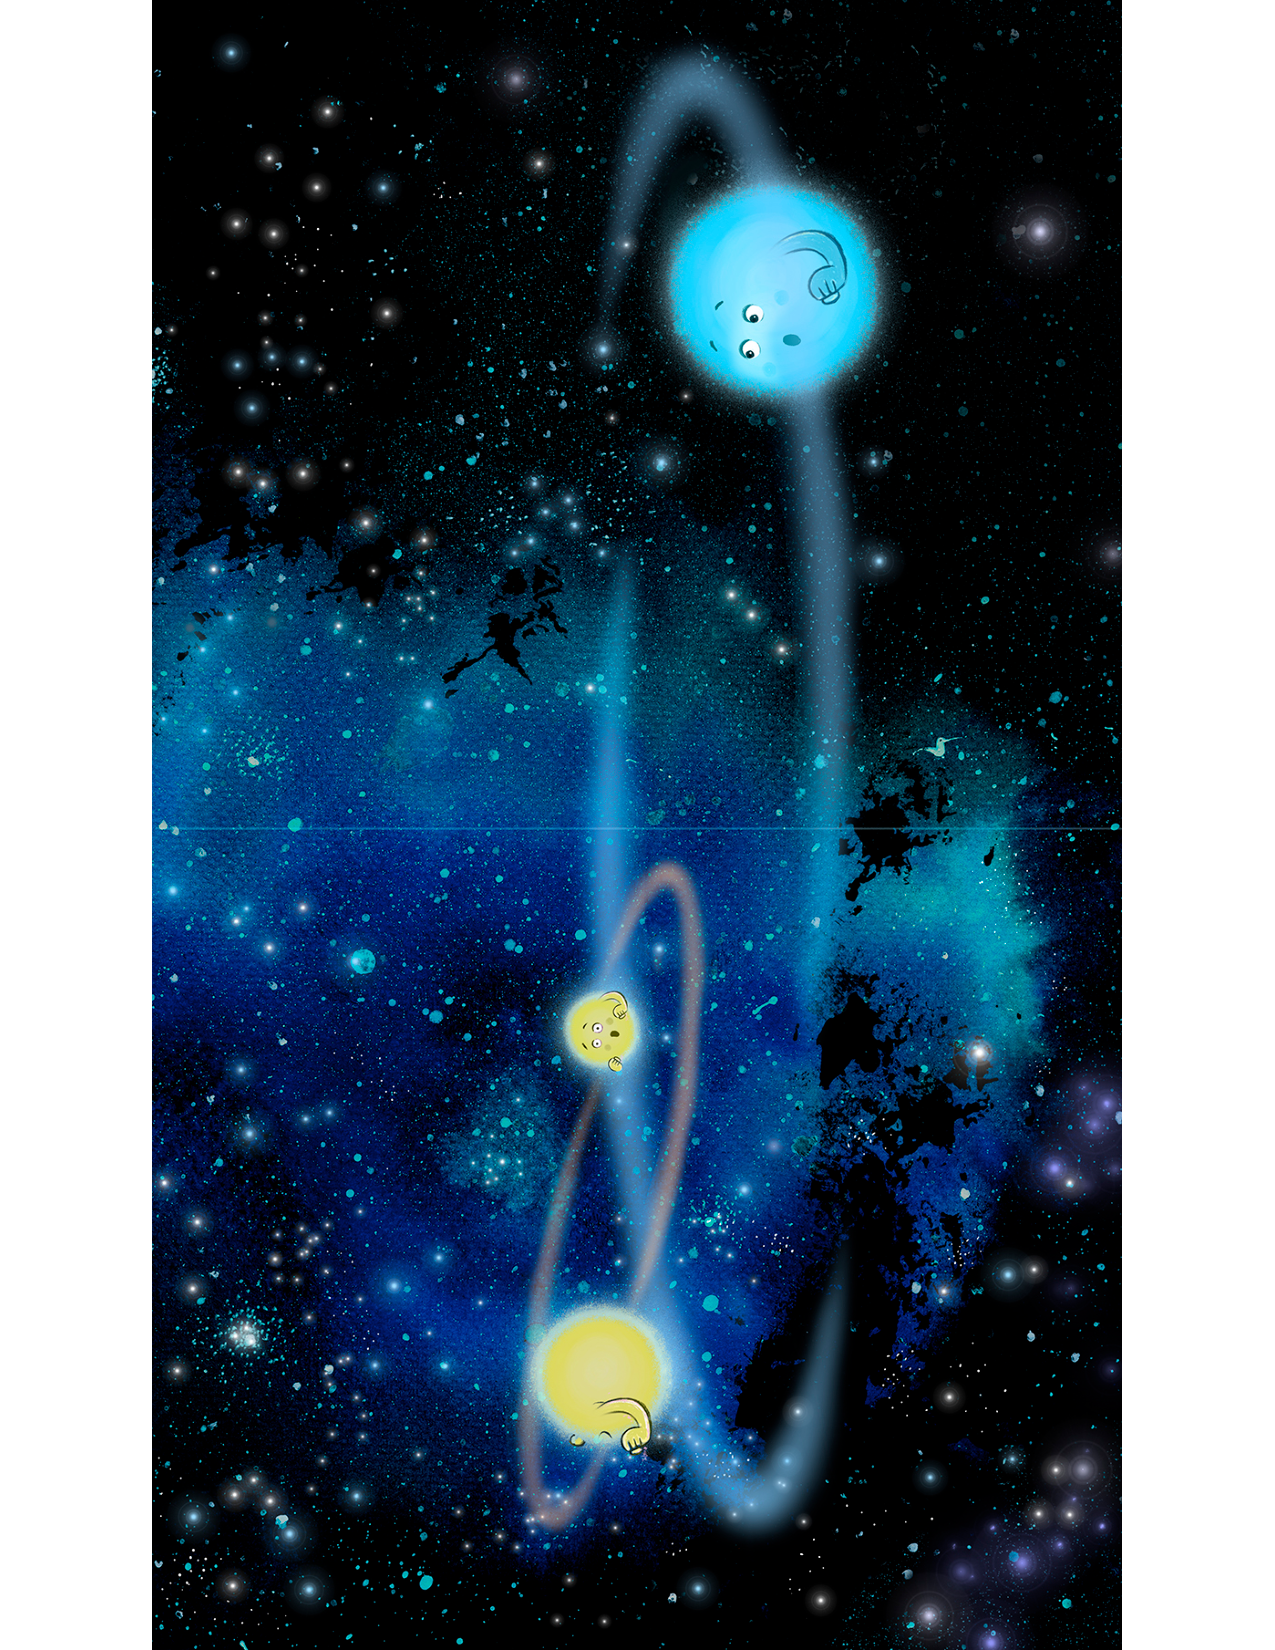
\includegraphics[width=\columnwidth,angle=270,origin=c]{ch3_1.pdf}
\caption{\rmtaygete~ and \rmalcyone, who together form the inner binary of a triple star system, after they have been informed by Celaeno that they will soon collide.  Illustration by Andre Pipe Oliva.
\label{fig:fig1}}
\end{figure}

\begin{figure}
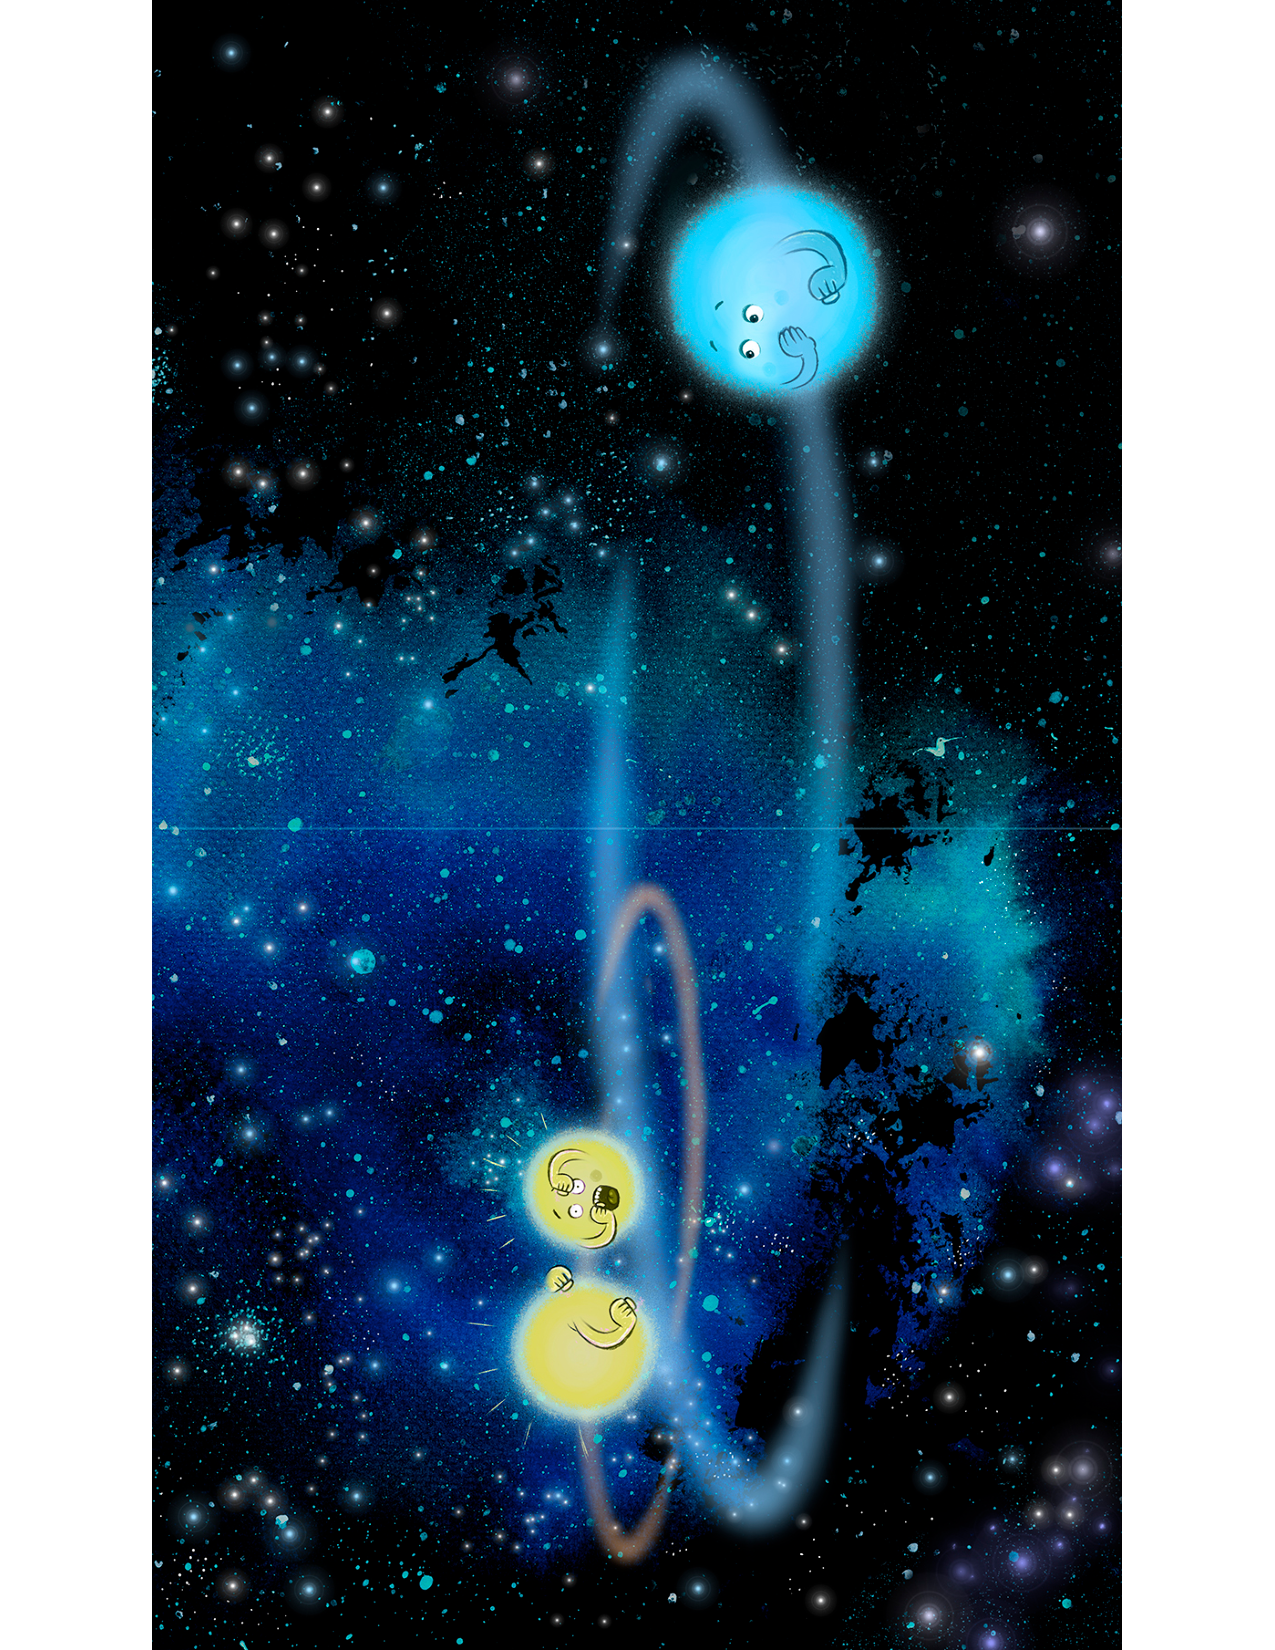
\includegraphics[width=\columnwidth,angle=270,origin=c]{ch3_2.pdf}
\caption{\rmtaygete~ and \rmalcyone, right before they collide.  Illustration by Andre Pipe Oliva. \note{From Adrian: I like it, but I wonder if the greyish inner orbit can be made to look more like it is highly eccentric. Now it looks the same as in the previous figure. }
\label{fig:fig1}}
\end{figure}

\par \nar Just then, \rmtaygete~ smashes in to \rmalcyone~ as they both re-approach their mutual periastron passage.  The collision is violent; the relative velocity is of order the sum of their local orbital speed, which is several hundred kilometers per second.  Needless to say, the sisters never stood a chance.  Their innards and organs (i.e., massive globs of hot gas) are flung violently away from the merging pair.  It is a grizzly scene.

\par \Celaeno Oh, Dear Lord!  I think I'm going to throw up.  SO MUCH PLASMA!  Gross, disgusting, and emotionally it's a lot to handle. ...Yep, here comes the vomit...

\par \nar \rmcelaeno~ suddenly vomits, spraying a particularly potent coronal mass ejection (or CME, for short) in to her immediate vicinity.  The vomited CME extends in an arc spanning about 120 degrees due to \rmcelaeno's rapid rotation rate.

\par \Celaeno Oooooooh my Gawd, they've got to be dead after that.  So gross!  

\par \nar \rmcelaeno~ nearly vomits a second time, but manages to stifle the urge.

\section{From the Ashes...} 

\par \Celaeno ...Uh...I guess I should check to see if everybody is okay? ...CAN YOU HEAR ME?!  ARE YOU STILL THERE?! 

\par \nar Gravity was in the process of taking the remains of what had once been \rmtaygete~ and \rmalcyone, and re-shaping them into a brand new star.  Formed from two stellar corpses, this new star was quickly turning out to be nearly twice as massive as each of his individual progenitors.  Suddenly, the product of this coalescence awoke.

%was spinning rapidly, but not for long; intense magnetic fields had been amplified during the collision and were rapidly spinning the new star to lower rotational frequencies.  A few millions years from now, all signs of the simultaneous deaths of two brothers, needed to give life to a new sister, will have vanished. 

\par \Lacedaemon Uh...Hello, there!  My name is...uh...\rmlacedaemon, I do believe.  I appear to be new to the scene...of which I know absolutely nothing about.  Where are we exactly?  Uh...\textit{What} are we?

\par \Celaeno Hello!  You are my new brother.  We are stars; spheres of gas and dust that contract after merging due to gravity into the configuration you see before you, which in turn rose the temperature in our cores \textit{a lot}.  We are slowly undergoing nuclear fusion in our bellies, converting hydrogen into helium and in the process emitting energy in the form of light or photons.  The outward momentum supplied by the photons provides the outward pressure we need to balance the inward force from gravity.  Mother called it ``hydrostatic equilibrium''.

\begin{figure}
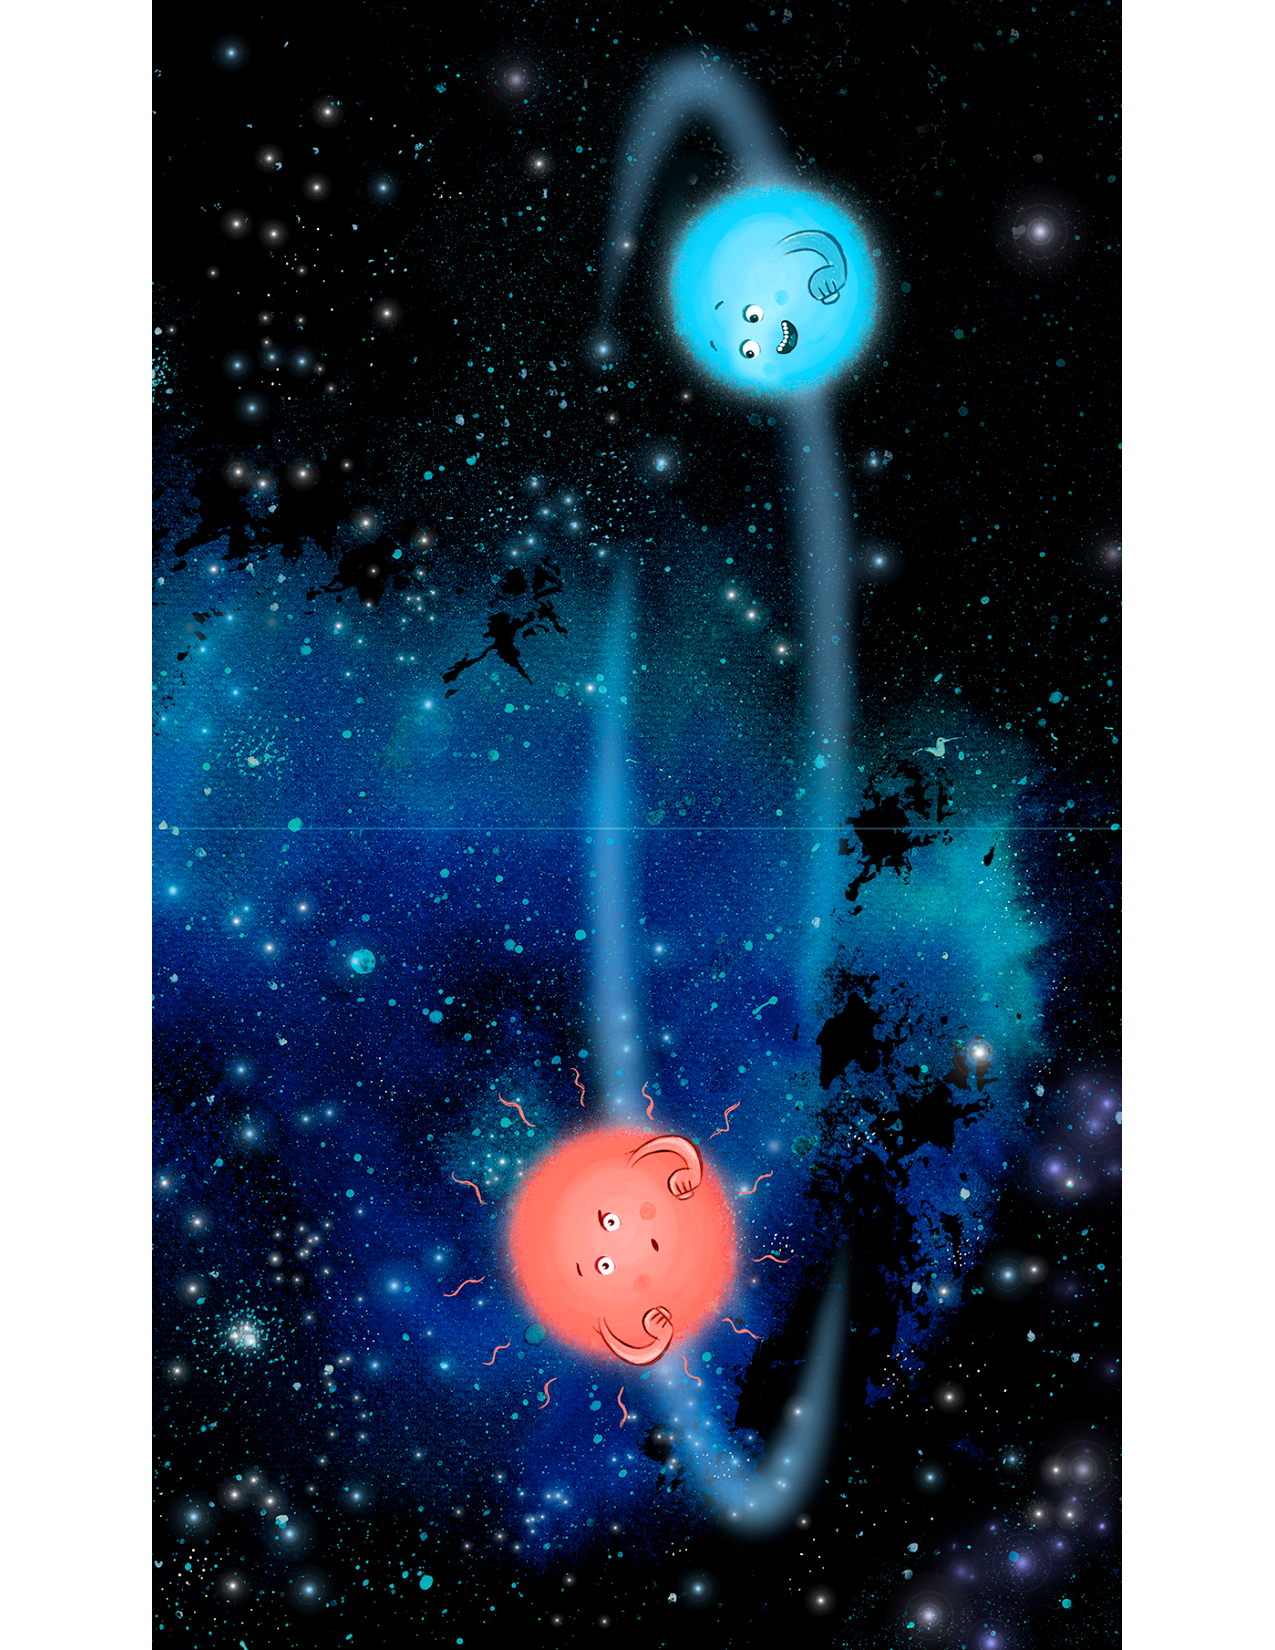
\includegraphics[width=\columnwidth,angle=270,origin=c]{ch3_3.pdf}
\caption{\rmlacedaemon~, formed from the remains of the merged \rmtaygete~ and \rmalcyone~, and his sister \rmcelaeno~.  Together, they now constitute a newly formed binary star system.  Illustration by Andre Pipe Oliva.
\label{fig:fig1}}
\end{figure}

\par \Lacedaemon Wow, that was a lot of very technical information.  Still, I appreciate it very much!  In fact, I'm quite impressed.  Now that you mention it, I'm starting to feel very balanced overall.  

\par \Celaeno I'm glad to hear it!

\par \Lacedaemon ...Well, except for this excess rotation I seem to be holding on to. And it goes right to the belly, let me tell you.  Wow, this bulge is really extending outward at my equator.  SUPER!  
%You look very svelt for a star, I must say.  I seem to be holding on to all this extra crud around my mid-center.  Rotational weight, that's the culprit.  Who would have guessed that angular momentum conservation would be this much work?

\par \nar \rmlacedaemon~ rolls his eyes to accentuate the sarcastic remark.

\par \Celaeno Don't worry, I've seen it lots of times before.  New stars spin down as they grow out of infancy.

\begin{comment}
%leveltwo or levelthree:
%\footnote{ANGULAR MOMENTUM CONSERVATION DISCUSSION, in the context of spin!}  
\begin{tcolorbox}[sharp corners, colback=blue!30, colframe=blue!80!blue, title=Torque]
\par \textcolor{blue}{DEFINE TORQUE.}.  
\end{tcolorbox}
\end{comment}


\par \Celaeno So, the ``belly'' will go away.  You'll settle in to a more sphere-like shape in no time.  You just have to radiate away the excess energy deposited within you from the kinetic energy of the collision.  I think the spinning down has something to do with ``magnetic fields'', or so I have heard.  As near as I can tell, this is some magical force that slows your spin rate down as you mature into a beautiful new star.

\par \Lacedaemon Hey, alright!  Good news.  I'm sold.  I mean, who doesn't appreciate spherical symmetry?  Weirdos, that's who.  Uh...So now what?

\par \nar \rmcelaeno~ liked her new brother, convinced she would appreciate having him around.

\par \Celaeno We focus on the journey ahead, of course.  Who knows where our fate will take us.  But now that we are free of our siblings, I suppose almost anything \textit{could} happen.  Here is hoping for good things!

\par \Lacedaemon  Wow, this is exciting!  Do you suppose we will run in to our other siblings?

\par \Celaeno Well, it's a big Galaxy out there, that much is for sure.  But, as I said, anything \textit{could} happen, especially given the long lives of stars.  

\par \Lacedaemon We have that going for us!  Wait...Just how long are we talking about?

\par \Celaeno Many millions or even billions of years.  In fact, I am guessing that somewhere out there are stars as old as the Galaxy itself.

\par \Lacedaemon Wow!  By the time I'm that old, I hope to have toured the entire Galaxy....Twice!

\par \Celaeno In that case, we had better get started.  The Galaxy sure isn't getting any smaller...

%A worried expression became evident on $\Celaeno's$ face.  
%
%\Lacedaemon  You look like you just saw something terrifying.  What's up?
%
%\Celaeno  Well, if you take our current trajectory through the Galaxy and propagate it forward through time, it looks to me like we are ultimately heading for the Galactic Center.
%
%\Lacedaemon  Great!  Wait... What is a ``Galactic Center''?
%
%\Celaeno  It is the very center of our Galaxy.  Here, a dense nuclear star cluster lives, jam packed with stars spanning all sort of masses and ages.  We are in the field of our Galaxy currently, where the mean stellar density is about 1 star per cubic parsec.  For example the distance separating the Sun and her next nearest neighbor, Proxima Centauri, is about a parsec.  But if you take the Sun and Proxima Centauri as they are observed, and drop them in to the very central regions of the nuclear cluster at the heart of our Galaxy, then more than 100 stars will fall between the pair.  The densities are that much higher.  
%
%\Lacedaemon  Wow.  That sounds crowded.  I bet you can hear \textit{everything} \textit{everyone} is doing, at any given moment.  *shudders*  
%
%\Celaeno But the really terrifying thing, if you ask me, is the super-massive black hole lurking at the heart of the nuclear cluster.    
%
%\Lacedaemon Super-massive black hole, you say?  What the hell is that?
%
%\Celaeno It is a dense dark object that does not emit light, typically way smaller than Jupter in size.  But it's total mass can range anywhere from 10$^6$ to 10$^{10}$ times the mass of the Sun.  In our own Milky Way, the super-massive black hole is known to be about 4 $\times$ 10$^6$ times the mass of the Sun.
%
%\Lacedaemon Holy cow!  That sounds....potentially violent.
%
%\Celaeno Uh... Yeah, it is.  Technically, if you wander too close to a super-massive black hole, it can eat you whole.  And, once inside its belly, you can never escape.
%
%\Lacedaemon  Oh, wonderful!  That doesn't sound even remotely terrifying...
%
%\Celaeno Um... And even if you don't get eaten, if you do wander close to a super-massive black hole, you are almost certainly going to get accelerated to extremely high velocities.  Like, we are talking thousands of kilometers per second.  
%
%\Lacedaemon  WHAT?!  Is that even possible?
%
%\Celaeno  Yep, such fast stars have definitely been seen whipping by in our very own Galaxy.  
%
%\Lacedaemon Well, this is all very terrifying.  How can we possibly prepare for a journey through the central nuclear star cluster of the Milky Way?
%
%\Celaeno Well, I'm going to take another nap, personally.  I figure we'll need to be fresh and alert, if nothing else.
%  
%
%\Lacedaemon Oh my gawd, you don't have a plan!  We are so going to die!
%
%$\Celaeno$ had already fallen asleep, and was now snoring loudly.



\section{Educational Material}

\begin{tcolorbox}[sharp corners, colback=red!30, colframe=red!80!blue, title=Box \refstepcounter{educhap3}\label{boxchap3:dynI}\ref{boxchap3:dynI} -- Orbital Dynamics I]
\par \textcolor{black}{As a first approximation, the motion of celestial objects such as stars is dictated by Newton's laws of motion. These laws state that the gravitational force on a body caused by another body is determined by the masses of the two bodies, and the separation between them (decreasing with increasing distance). Something like a {\it body} may sound abstract (and a bit morbid!), but it means a point mass, that is, an object with all of its mass concentrated into a single point in space. It turns out that this is a good description if the physical object that the body represents is (close to) spherical, which is the case for most stars in the Universe (exceptions exist for some highly rotating stars, and stars in close binaries which are affected by their companion). \\ \\
To describe the motion of a system with an arbitrary number of bodies, one computes the net force on each body by adding the gravitational force from all pairs with all other bodies (known as the {\it superposition principle}). The resulting equations of motion can only be solved in closed analytic form (that is, on pen and paper) when the number of bodies is just two (one of Newton's most renowned discoveries). When the number of bodies is larger, exact solutions can only be found in specific cases. 
}
%GIVE THE READER THE LOWEST LEVEL EXPLANATION OF ORBITAL DYNAMICS POSSIBLE.}.  
\end{tcolorbox}

\begin{tcolorbox}[sharp corners, colback=blue!30, colframe=blue!80!blue, title=Box \refstepcounter{educhap3}\label{boxchap3:dynII}\ref{boxchap3:dynII} -- Orbital Dynamics II]
\par \textcolor{black}{Consider two bodies with masses $m_1$ and $m_2$. Their position vectors are denoted with $\myvec{R}_1$ and $\myvec{R}_2$, respectively. The gravitational force on body 1 is given by
\begin{align}
\label{Chap3:Eq:F_1_vec}
\myvec{F}_{1} = - \gconst m_1m_2 \frac{\myvec{R}_1 - \myvec{R}_2}{|| \myvec{R}_1 - \myvec{R}_2||^3}.
\end{align}
\note{A.S.H.: Have we defined $\gconst$ already by this point?} Newton's Third Law states that the force on body 2 is simply equal in magnitude but opposite in direction to that of the force on body 1, that is,
\begin{align}
\myvec{F}_{2} = - \myvec{F}_{1}.
\end{align}
From this, it is easy to see that the net force on the system is zero: $\myvec{F}_1 + \myvec{F}_2 = \myvec{0}$. \\ \\
If there are more than two bodies, we need to apply the superposition principle: for each body $i$ in the system, we compute the total force on that body by considering pairs $(i,j)$ with all other bodies and sum the force for each pair:
\begin{align}
\label{Chap3:Eq:GravForcei}
\myvec{F}_i = -\gconst m_i \sum_{\substack{j=1 \\ j\neq i}}^{N} m_j \frac{ \myvec{R}_i - \myvec{R}_j}{|| \myvec{R}_i - \myvec{R}_j||^3}.
\end{align}
Note that, in the summation over $j$, we must make sure that $j\neq i$, since we would otherwise double count pairs of bodies. Newton's Second Law for $\myvec{R}_i$ reads
\begin{align}
\label{Chap3:Eq:Newton_Second}
\myvec{F}_i = m_i \myvec{a}_i = m_i \frac{\mathrm{d}^2 \myvec{R}_i}{\mathrm{d} t^2},
\end{align}
where $t$ is the time, and $\myvec{a}_i$ is the acceleration of body $i$. In Newtonian dynamics, the mass $m_i$ that appears in \Eq~(\ref{Chap3:Eq:Newton_Second}), the {\it inertial mass}, is the same as the {\it gravitational mass} $m_i$ that appears in \Eq~(\ref{Chap3:Eq:GravForcei}) (this is known as the {\it equivalence principle}). Therefore, the acceleration of body $i$ does not depend on its own mass $m_i$, and is given by
\begin{align}
\label{Chap3:Eq:EOM}
\frac{\mathrm{d}^2 \myvec{R}_i}{\mathrm{d} t^2} = - \gconst \sum_{\substack{j=1 \\ j\neq i}}^{N} m_j \frac{ \myvec{R}_i - \myvec{R}_j}{|| \myvec{R}_i - \myvec{R}_j||^3}.
\end{align}
}.  
\end{tcolorbox}


\begin{tcolorbox}[sharp corners, colback=red!30, colframe=red!80!blue, title=Box \refstepcounter{educhap3}\label{boxchap3:incl}\ref{boxchap3:incl} -- Orbital Inclination]
\par \textcolor{black}{ Although the orbit of a two-body system lies within a two-dimensional plane, when more bodies (and therefore orbits) are involved, it is useful to define the inclination of an orbit relative to a reference frame, or to another orbit. In observational astronomy, inclinations are usually defined with respect to the {\it sky plane}. This means that the `inclination' is the angle between the orbital plane, and the plane of the sky. In the case of hierarchical triple systems with an inner and an outer orbit, one can define the {\it mutual} or {\it relative} inclination between the two orbits. When the latter is zero, the orbits are coplanar. A mutual inclination of 90 degrees means the orbits are perpendicular. When the mutual inclination is 180 degrees, then the orbits are again coplanar, but the bodies are moving in opposite directions relative to each other. }  
\end{tcolorbox}



%levelone
%or leveltwo?
\begin{tcolorbox}[sharp corners, colback=red!30, colframe=red!80!blue, title=Box \refstepcounter{educhap3}\label{boxchap3:ecc}\ref{boxchap3:ecc} -- Orbital Eccentricity]
\par \textcolor{black}{The Earth orbits about the Sun on a roughly circular orbit, such that its distance from the Sun does not change much over the course of a year\footnote{Seasonal changes are mostly driven by the Earth's non-zero {\it obliquity}: its rotation axis is tilted at about $23.5^\circ$ with respect to the orbital plane. This means that during one half of the year, more sunlight arrives at the southern hemisphere compared to the north (Summer in the southern hemisphere; Winter in the north), whereas this is reversed during the other half of the year. }. Hence, a reasonable approximation here for most purposes is that the Earth's orbital eccentricity is nearly zero, or $e \approx 0$.  This is not the case for every orbit, however.  Some orbits have non-zero eccentricities, orbiting their centers of mass on elliptic orbits.  In the limit $e \rightarrow 1$, the two bodies orbit each along a straight line, and are doomed to crash into each other and collide (if they have not already experienced other effects such as strong tidal evolution before reaching $e \rightarrow 1$).}
\end{tcolorbox}


\begin{tcolorbox}[sharp corners, colback=red!30, colframe=red!80!blue, title=Box \refstepcounter{educhap3}\label{boxchap3:periapo}\ref{boxchap3:periapo} -- Periapsis and apoapsis]
\par \textcolor{black} {\note{A.S.H.: I changed `apoastron/periastron' to `apoapsis/periapsis' since the latter are general terms. OK?} The part of furthest separation in the trajectory of an orbiting body is called ``apoapsis'', and corresponds to where along an eccentric orbit the orbital velocity is at a minimum. The part of closest approach of the trajectory of an orbiting body is called ``periapsis'', and corresponds to where along an eccentric orbit the orbital velocity is at a maximum. In a circular orbit, the relative orbital distance is always the same, hence both the periapsis and apoapsis are equal to the constant relative orbital separation, and the orbital speed (i.e., magnitude of the velocity) is constant. }
\end{tcolorbox}



\begin{tcolorbox}[sharp corners, colback=blue!30, colframe=blue!80!blue, title=Box \refstepcounter{educhap3}\label{boxchap3:dynIII}\ref{boxchap3:dynIII} -- Orbital Dynamics III]
\par \textcolor{black}{As alluded to before, Newton's equations of motion can be solved analytically for two bodies. We will briefly discuss this solution here. \\ \\
First, we will show that the problem of two bodies (with two position vectors, $\myvec{R}_1$ and $\myvec{R}_2$) can be reduced to effectively a one-body problem (with just one position vector, $\myvec{r}$). Let $\myvec{r} \equiv \myvec{R}_1 - \myvec{R}_2$. If we take Newton's equation of motion for $\myvec{R}_1$ and $\myvec{R}_2$ and subtract them, we get
\begin{align}
\label{Chap3:Eq:2b_EOM_r}
\ddot{\myvec{r}} &= \ddot{\myvec{R}}_1 - \ddot{\myvec{R}}_2 =  -\gconst (m_1+m_2)  \frac{\myvec{r}}{r^3}.
\end{align}
Here, we use dots to denote time derivatives (so two dots means taking the second time derivative). Once we know how $\myvec{r}$ evolves, that is, once we have the solution $\myvec{r}(t)$, we can get the motion of the individual bodies 1 and 2 through the relations
\begin{subequations}
\label{Chap3:Eq:R_r_relations}
\begin{align}
\myvec{R}_1 &= \myvec{r}_\mathrm{CM} + \frac{m_2}{m_1+m_2} \myvec{r}; \\
\myvec{R}_2 &= \myvec{r}_\mathrm{CM} - \frac{m_1}{m_1+m_2} \myvec{r}.
\end{align}
\end{subequations}
Here, $\myvec{r}_\mathrm{CM}$ is the {\bf center of mass} position vector given by
\begin{align}
\label{Chap3:Eq:r_CM_def}
\myvec{r}_\mathrm{CM} \equiv \frac{m_1 \myvec{R}_1 + m_2 \myvec{R}_2}{m_1+m_2}.
\end{align} 
There are various ways to arrive at the solution for $\myvec{r}(t)$. Here, we will not discuss how to derive the result, but just mention it. Note that the solution can be checked by plugging it into the equation of motion, \Eq~(\ref{Chap3:Eq:2b_EOM_r}). The solution can be written in the general form:
\begin{align}
\label{Chap3:Eq:r_sol}
\myvec{r}(t) = r(t) \left [ \cos(\TA) \, \unit{e} + \sin(\TA) \, \unit{q} \right ].
\end{align}
Here, $r(t)$ is the magnitude of $\myvec{r}(t)$ given by
\begin{align}
r(t) = \frac{a \left(1-e^2\right)}{1 + e \cos (\TA)},
\end{align}
with $a$ and $e$ the orbital semimajor axis and eccentricity, respectively (they are constants of the motion), whereas $\TA=\TA(t)$ is the {\it true anomaly} that characterizes the orbital phase ($\TA$ varies with time, and in a non-linear fashion). Note that the closest approach in the orbit, the periapsis, corresponds to $\TA=0$ with separation $r_\mathrm{p} = a(1-e)$. The largest separation (apoapsis) is reached when $\TA=\pi$, with $r_\mathrm{a} = a(1+e)$. \\ \\
There are two more constant quantities in \Eq~(\ref{Chap3:Eq:r_sol}): $\unit{e}$ and $\unit{q}$. The former, $\unit{e}$, is the (unit) {\bf eccentricity vector} that points along the {\bf line of apsides}, the line connecting the periapsis (point of closets approach in the relative orbit) and apoapsis (point of furtest approach in the relative orbit). The vector $\unit{q}$ is perpendicular to both $\unit{e}$ and $\unit{l}$, where $\unit{l}$ points along the angular momentum of the orbit. In vector notation: $\unit{q} = \unit{l} \times \unit{e}$. Note that $\unit{e}$, $\unit{q}$, and $\unit{l}$ are all constant in the two-body problem. }
\end{tcolorbox}

\begin{tcolorbox}[sharp corners, colback=blue!30, colframe=blue!80!blue, title=Box \ref{boxchap3:dynIII} -- Orbital Dynamics III (continued)]
\par \textcolor{black}{The relation between physical time $t$ and the true anomaly $\TA$ is described by the {\bf Kepler equation}. First, we need to introduce another angle which describes the orbital phase and which is closely related to the true anomaly: the {\bf eccentric anomaly}, $\EA$. The relation between $\TA$ and $\EA$ is given by
\begin{align}
\label{Chap3:Eq:EA_to_TA}
\cos(\TA) = \frac{\cos(\EA) - e}{1 - e \cos(\EA)}; \qquad \sin(\EA) = \sqrt{1-e^2} \frac{\sin(\TA)}{1+e\cos(\TA)}.
\end{align}
The Kepler equation relates $\EA$ (and hence $\TA$) to time $t$ according to
\begin{align}
\label{Chap3:Eq:kep_eq}
\EA - e \sin(\EA) = n(t-\tau).
\end{align}
Here, $n$ is the {\bf mean motion} given by
\begin{align}
n \equiv \frac{2\pi}{P} = \sqrt{\frac{G(m_1+m_2)}{a^3}},
\end{align}
where $P$ is the {\bf orbital period}, given by
\begin{align}
\label{Chap3:Eq:kepl}
P = 2 \pi \sqrt{\frac{a^3}{G(m_1+m_2)}}.
\end{align}
Furthermore, $\tau$ is the time of periapsis passage, i.e, a reference time at which the orbit passes periapsis. The combination $n t$ (or $nt - n\tau$) is known as the {\bf mean anomaly} $\MA$. We note that \Eq~(\ref{Chap3:Eq:kep_eq}) has no simple solutions for $\EA$ for a given $t$ (except in the trivial case of circular orbits, $e=0$). Generally, it has to be solved numerically, for example, by means of {\bf Newton iteration}.}
\end{tcolorbox}

\begin{tcolorbox}[sharp corners, colback=green!30, colframe=green!80!blue, title=Box \refstepcounter{educhap3}\label{boxchap3:dynIV}\ref{boxchap3:dynIV} -- Orbital Dynamics IV]
\par \textcolor{black}{In Box~\ref{boxchap3:dynIII}, we discussed the analytic solution to the two-body problem and described it in terms of the orbital vectors, $\unit{e}$ and $\unit{q}$ (or, equivalently, $\unit{e}$ and $\unit{l}$. Another way of describing the orbital orientation is using {\bf orbital angles} (which of the two is better to use, i.e., orbital vectors or orbital angles, depends on the problem). The orbital angles (in addition to $\TA$, $\EA$ or $\MA$, which describe the orbital phase) are the inclination $i$, the {\bf argument of periapsis} $\omega$ and the {\bf longitude of the ascending node} $\Omega$. These angles are equivalent to the `Euler' angles which describe the orientation of an object in a coordinate system. \note{A.S.H.: Do we want to include a figure to illustrate orbital elements?}. \\ \\
The following relations exist between the orbital elements and the orbital vectors. First, to compute the elements from the vectors, we have:
\begin{align}
\cos(i) = \unit{z} \cdot \unit{l},
\end{align}
for the inclination. Here, $\unit{z}$ is just the unit $z$-direction in the coordinate system. For any two-body system, the unit orbital angular momentum vector $\unit{l}$ at any time is given by
\begin{align}
\unit{l} = \frac{ \myvec{r} \times \myvec{v}}{||\myvec{r} \times \myvec{v} ||}.
\end{align}
To get the longitude of the ascending nodes $\Omega$, we define the so-called ascending node vector, $\unit{\Omega}$:
\begin{align}
\unit{\Omega} = \unit{z} \times \unit{l}.
\end{align}
We then have
\begin{align}
\cos(\Omega) = \unit{x} \cdot \unit{\Omega}; \qquad \sin(\Omega) = \unit{y} \cdot \unit{\Omega}.
\end{align}
The argument of pericenter, $\omega$, is determined by
\begin{align}
\cos(\omega) = \unit{e} \cdot \unit{\Omega}; \qquad \sin(\omega) = -\unit{q} \cdot \unit{\Omega}.
\end{align}
%Finally, the true anomaly is determined by
%\begin{align}
%\cos(\TA) = \unit{e} \cdot \unit{r};  \qquad \sin(\TA) = \unit{q} \cdot \unit{r}.
%\end{align}
The reverse operation (from orbital elements to orbital vectors) is described by
\begin{subequations}
\label{Chap3:Eq:elements_to_vec}
\begin{align}
\nonumber \unit{e} &= \left [ \cos(\Omega) \cos(\omega) - \sin(\Omega) \sin(\omega) \cos(i) \right ] \unit{x} + \left [ \sin(\Omega) \cos(\omega) \right. \\
&\quad \left. + \cos(\Omega) \sin(\omega) \cos(i) \right ] \unit{y} + \sin(\omega) \sin(i) \, \unit{z}; \\
\nonumber \unit{q} &= \left [ -\cos(\Omega) \sin(\omega) - \sin(\Omega) \cos(\omega) \cos(i) \right ] \unit{x} + \left [ -\sin(\Omega) \sin(\omega) \right. \\
&\quad \left. + \cos(\Omega) \cos(\omega) \cos(i) \right ] \unit{y} + \cos(\omega) \sin(i) \, \unit{z}.
\end{align}
\end{subequations}
}
\end{tcolorbox}

\begin{tcolorbox}[sharp corners, colback=green!30, colframe=green!80!blue, title=Box \ref{boxchap3:dynIV} -- Orbital Dynamics IV (continued)]
\par \textcolor{black}{As also discussed in Box~\ref{boxchap3:dynIII}, the {\it Kepler} equation cannot be solved analytically in general. A useful method to solve it numerically is using {\bf Newton iteration}. The latter is formulated as follows: let $f(x)$ be a function of $x$, and we wish to know the value of $x=x_0$ such that $f(x_0)=0$. We can then apply an iterative scheme based on the derivative of $f(x)$: 
\begin{align}
x_{n+1} = x_n - \frac{f(x_n)}{f'(x_n)},
\end{align}
where the prime denotes derivative with respect to $x$. In our case, to solve \Eq~(\ref{Chap3:Eq:kep_eq}), we can write $f(\EA) = \EA - e \sin(\EA) - \MA$ where $\MA = n(t-\tau)$, such that
\begin{align}
\EA_{n+1} = \EA_n - \frac{\EA_n - e \sin(\EA_n) - \MA}{1 - e \cos(\EA_n)}.
\end{align}
}
\end{tcolorbox}


\begin{tcolorbox}[sharp corners, colback=blue!30, colframe=blue!80!blue,  title=Box \refstepcounter{educhap3}\label{boxchap3:stab}\ref{boxchap3:stab} -- Stability of hierarchical triples]
\par \textcolor{black}{ In a hierarchical triple system, two objects orbit each other in a relatively tight orbit (the ``inner orbit''), whereas a third object orbits the former two objects' center of mass in a wider orbit (the ``outer orbit''). If the inner orbit is sufficiently more compact than the outer orbit, the system can remain stable on long time-scales. On short time-scales, the orbits are nearly Keplerian. At any given time, one can define ``osculating'' orbital elements. If the third object were instantaneously removed, the inner orbit would be perfectly Keplerian and its orbital elements would be the osculating elements. \\ \\
It is generally hard to predict exactly whether or not a given hierarchical triple is stable or not (i.e., without integrating the equations of motion numerically). First, there is no unique way of defining stability. In a stable system, the energies (and hence semimajor axes) of the inner and outer orbits do not change systematically over time. However, they can change on shorter time-scales as the bodies move in their nearly-Keplerian orbits. These changes in the (osculating) orbital elements increase in magnitude as the triple becomes more compact (i.e., the inner and outer orbital separations become more comparable and so the tertiary star aproaches the inner binary at closer and closer periapsis distances).  Also, the notion of stability depends on what timescale one requires the triple to be stable, since chaos in three-body systems can lead to destabilization of the system on timescales that are much longer than the orbital timscales. \\ \\
Nevertheless, several usuful analytic criteria have been developed that can be used to predict stability of a given system. A well known and widely used criterium is that of Marding and Aarseth \citep{} \note{Missing reference -- bibliography needs to be set up}, which reads \\ \\
\begin{align}
\frac{a_2(1-e_2)}{a_1} > 2.8 \left [ (1 + q_2) \frac{1+e_2}{(1 - e_2)^{1/2}} \right ]^{2/5} \left (1 - \frac{0.3 i_{\mathrm{rel}}}{180} \right ).
\end{align}
Here, subscripts `1' and `2' refer to the the inner and outer orbits, respectively. The mass ratio $q_2$ is defined as $q_2 \equiv m_3/(m_1+m_2)$, where $m_1$ and $m_2$ are the masses of the two components in the inner binary, and $m_3$ is the mass of the third body. The mutual inclination between the inner and outer orbits is $i_{\mathrm{rel}}$, and it affects stability in addition to the semimajor axes and eccentricities. This criterion works well for systems in which the three masses are not too distinct from each other. For other cases (e.g., two planets around a star), other criteria are more appropriate (not discussed here). 
}
\end{tcolorbox}


\begin{tcolorbox}[sharp corners, colback=blue!30, colframe=blue!80!blue, title=Box \refstepcounter{educhap3}\label{boxchap3:dynV}\ref{boxchap3:dynV} -- Orbital dynamics V]
\par \textcolor{black}{Even if a triple system is hierarchical and long-term stable, its inner and outer orbits can still change over time due to {\bf torques} that the inner and outer orbits exert on each other, leading to {\bf angular momentum exchange}. In the stellar context when all three bodies have similar masses, the angular momentum budget is dominated by the outer orbit, and the torques have the largest effect on the inner orbit. The angular momentum variations occur periodically; if the inner and outer orbits are initially sufficiently inclined, then the inner orbit eccentricity oscillates and can reach high values; these oscillations are known as  {\bf von Zeipel-Lidov-Kozai (ZLK)} oscillations. They have important implications in a large range of astrophysical systems. Examples beyond stellar triple systems include (but are not limited to) binary systems in galactic nuclei with a central massive black hole, triple supermassive black holes, planets in binary star systems, and binary asteroids.
A very useful technique to study the long-term evolution in stable hierarchical triples is the {\bf secular} approximation, in which the Hamiltonian of the system is expanded in the (small) ratio of the inner to outer orbital separation. One then averages over the inner and outer orbits, which greatly simplifies the equations of motion. After applying this technique, as a first approximation (lowest expansion order, assuming one of the bodies in the inner binary is massless, and that the inner orbit has zero initial eccentricity), the {\bf maximum eccentricity} reached is given by
\begin{align}
\label{eq:ZLK_emax}
e_\mathrm{max} = \sqrt{1-\frac{5}{3}\cos^2 (i_\mathrm{rel})},
\end{align}
where $i_\mathrm{rel}$ is the initial relative inclination angle between the inner and outer orbits. This shows that $e_\mathrm{max}$ is sensitively dependent on $i_\mathrm{max}$; in particular,  eccentricity excitation occurs only if $\cos(i_\mathrm{rel}) < \sqrt{3/5}$ (so $39.23^\circ \lesssim i_\mathrm{rel} \lesssim 140.77^\circ$), and $e_\mathrm{max} \rightarrow 1$ as $i_\mathrm{max} \rightarrow 90^\circ$. As a first approximation, the {\bf period} of the oscillations is given by
\begin{align}
T_\mathrm{ZLK} \approx \frac{P_2^2}{P_1} \frac{m_1+m_2+m_3}{m_3} \left(1-e_2^2 \right )^{3/2},
\end{align}
where $P_\mathrm{in}$ and $P_\mathrm{out}$ are the inner and outer orbital periods, respectively. 
The above expressions are first approximations that are stricitly valid only in rather simplified cases. In the more general case, the dynamics are more complicated. When higher-order effects in the expansion are taken into account (in particular, octupole-order terms), then the long-term evolution can be {\bf chaotic}, and much higher eccentricities can be reached than implied by \Eq~(\ref{eq:ZLK_emax}). Specifically, octupole-order terms start to become important when
\begin{align}
\epsilon_\mathrm{oct} = \frac{|m_1-m_2|}{m_1+m_2} \frac{a_1}{a_2} \frac{e_2}{1-e_2^2} \gtrsim 10^{-4}.
\end{align}
Furthermore, ZLK oscillations can be {\bf quenched} if additional {\bf short-period forces} (forces that depend very sensitively on separation) act in the inner binary which lead to additional apsidal motion. These could arise, e.g., because of relativistic corrections, tidal bulges, or stellar rotation. Generally, this quenching occurs if the time-scale of apsidal motion due to short-range forces, $T_\mathrm{SRF}$, is significantly shorter than the ZLK time-scale, i.e., $T_\mathrm{SRF} \ll T_\mathrm{ZLK}$. 
}  
\end{tcolorbox}

%levelthree:
\begin{tcolorbox}[sharp corners, colback=green!30, colframe=green!80!blue, title=Box \refstepcounter{educhap3}\label{boxchap3:dynVI}\ref{boxchap3:dynVI} -- Orbital dynamics VI]
\par \textcolor{black}{Here, we discuss some analytical aspects of ZLK oscillations in more detail. The Hamiltonian of the hierarchical three-body system can be written in terms of the inner and outer orbital separations $\myvec{r}_1$ and $\myvec{r}_2$ as
\begin{align}
\label{eq:Htriplegen}
\nonumber \mathcal{H} &= T+V = - \frac{\gconst m_1m_2}{2a_1} - \frac{\gconst(m_1+m_2)m_3}{2 a_2} \\
&\quad - \frac{\gconst m_3}{r_2} \sum_{n=2}^\infty \mathcal{M}_n \left ( \frac{r_1}{r_2} \right )^n \widetilde{P}_n(\cos \Phi).
\end{align}
The first two terms represent the binding energies of the inner and outer orbits, respectively, and the remaining terms in the second line represent the {\bf perturbing function} that describes how the orbits evolve on time-scales (much) longer than the orbital time-scales (here, we assumed that the orbits are Keplerian on short time-scales in relation to the terms in the first line). The dimensionless mass parameter $\mathcal{M}_n$ is given by
\begin{align}
\mathcal{M}_n \equiv \frac{m_1 m_2}{m_1+m_2}\frac{m_1^{n-1} - (-m_2)^{n-1}}{(m_1+m_2)^{n-1}}.
\end{align}
Furthermore, $\widetilde{P}_n(x)$ is the $n^\mathrm{th}$ Legendre polynomial, and $\Phi$ is the (instantaneous) angle between $\myvec{r}_1$ and $\myvec{r}_2$. \\ \\
Truncating the expansion in \Eq~(\ref{eq:Htriplegen}) to $n=2$ (the {\bf quadrupole} order) and averaging over both inner and outer orbits, the Hamiltonian can be written as\footnote{There are cases when this `double' averaging is {\bf not} justified, i.e., it can happen that the time-scale on which orbits evolve is shorter than one of the orbital periods in the system. One notable example of this is the {\bf evection resonance}, when the time-scale for the inner orbit to precess due to the torque of the third body is comparable to the outer orbital period, potentially leading to additional eccentricity excitation. }
\begin{align}
\label{eq:Htriplequadav}
\nonumber \langle \mathcal{H}_\mathrm{quad}\rangle &= C_\mathrm{quad} \left [ \left (2 + 3 e_1^2 \right ) \left (3 \cos^2(i_\mathrm{rel}) - 1 \right ) \right. \\
&\quad \left. + 15 e_1^2 \sin^2(i_\mathrm{rel}) \cos(2\omega_1) \right ].
\end{align} 
Here, 
\begin{align}
C_\mathrm{quad} \equiv \frac{1}{16} \frac{\gconst m_1m_2m_3}{(m_1+m_2) \, a_\mathrm{out}} \left (\frac{a_1}{a_2} \right )^2 \left (1 - e_2^2 \right )^{-3/2},
\end{align}
and $\omega_1$ is the inner orbit argument of periapsis. Note that we here switched to {\bf orbital elements} to describe the orbital orientations. Also, we defined our orbital elements with respect to the {\bf invariable plane}, which is a plane perpendicular to the total angular momentum vector (which we assume is constant).
}  
\end{tcolorbox}

\begin{tcolorbox}[sharp corners, colback=green!30, colframe=green!80!blue, title=Box \ref{boxchap3:dynVI} -- Orbital dynamics VI (continued)]
\par \textcolor{black}{
Generally, from a given Hamiltonian, the {\bf equations of motion} read
\begin{align}
\label{eq:Hameq}
\left \{ \begin{array}{lll}
\displaystyle \dot{L}_j &= \displaystyle \frac{\partial \mathcal{H}}{\partial \TA_j}; & \dot{\TA}_j = \displaystyle - \frac{\partial \mathcal{H}}{\partial L_j}; \\
\displaystyle \dot{G}_j &= \displaystyle \frac{\partial \mathcal{H}}{\partial \AP_j}; & \dot{\AP}_j = \displaystyle - \frac{\partial \mathcal{H}}{\partial G_j}; \\
\displaystyle \dot{H}_j &= \displaystyle \frac{\partial \mathcal{H}}{\partial \LAN_j}; & \dot{\LAN}_j = \displaystyle - \frac{\partial \mathcal{H}}{\partial H_j}. \\
\end{array} \right.
\end{align}
The coordinates used are the {\bf Delaunay elements}; in particular, $L_j$, $G_j$, and $H_j$ are related to the orbital angular momentum: $L_j = \mu_j \sqrt{\gconst M_j a_j}$ is the circular orbital angular momentum, $G_j = L_j \sqrt{1-e_j^2}$ the general angular momentum, and $H_j = G_j \cos (i_j)$ the $z$-component of the angular momentum. Here, $\mu_j$ is the reduced mass, which is $\mu_1 = m_1m_2/M_1$ and $\mu_2 = m_3 M_1/M_2$ with $M_1 \equiv m_1+m_2$, and $M_2 \equiv m_1+m_2+m_3$. The {\bf conjugate} coordinates to the momenta $L_j$, $G_j$, and $H_j$ are the true anomaly $\TA_j$, the argument of periapsis $\AP_j$, and the longitude of the ascending node $\LAN_j$. \\ \\
From \Eq~(\ref{eq:Htriplequadav}), it is clear that the hierarchical three-body Hamiltonian at the quadrupole order is independent of $\AP_2$, which immediately implies that the {\bf outer orbital eccentricity $e_2$ is constant}. This feature disappears when higher-order terms are included (although, in systems with similar masses, the outer orbital eccentricity typically changes very little, unless the system is not very hierarchical). \\ \\
Furthermore, \Eq~(\ref{eq:Htriplequadav}) does not show a dependence on either $\LAN_j$. One needs to be very careful when interpreting this: it turns out that the dependence of the Hamiltonian on $\Omega_j$ is actually through the combination $\LAN - \LAN_2 \equiv \Delta \LAN$. In the coordinate frame that we considered, $\Delta \LAN = \pi$ always, meaning that the explicit dependence on the $\Omega_j$ is removed. However, the Hamiltonian still technically depends on the $\LAN_j$, hence the conjugate momenta $H_j$ are {\bf not generally conserved}. \\ \\
We can get further insight from \Eq~(\ref{eq:Htriplequadav}) by using energy and angular momentum conservation. If we restrict to the quadruple order, energy conservation simply means that \Eq~(\ref{eq:Htriplequadav}) is constant. Furthermore, angular momentum conservation implies there exists a relation between the eccentricities and the mutual inclination. Specifically, the total orbital angular momentum of the triple can be written as
\begin{align}
\label{eq:AM_triple}
G_\mathrm{tot}^2 = L_1^2 \left(1-e_1^2 \right ) + L_2^2 \left(1-e_2^2 \right ) + 2L_1 L_2 \sqrt{1-e_1^2} \sqrt{1-e_2^2} \cos i_\mathrm{rel}.
\end{align}}
\end{tcolorbox}

\begin{tcolorbox}[sharp corners, colback=green!30, colframe=green!80!blue, title=Box \ref{boxchap3:dynVI} -- Orbital dynamics VI (continued)]
\par \textcolor{black}{
At the quadrupole-order approximation, $e_2$ is constant. If we furthermore assume the inner circular angular momentum $L_1$ is small compared to the outer $L_2$ (the {\bf test particle limit}), then \Eq~(\ref{eq:AM_triple}) simply states that
\begin{align}
\label{eq:cZLK}
C_\mathrm{ZLK} \equiv \sqrt{1-e_1^2} \cos i_\mathrm{rel}
\end{align}
is constant. This is characteristic of (classical) ZLK oscillations.
\begin{minipage}[t]{0.5\linewidth}
    \vspace*{0pt}
        \includegraphics[width=2\columnwidth,angle=0,origin=c]{ZLK_ham}
        \captionof{figure}{Phase-space trajectories describing ZLK oscillations. }\label{fig:ZLK_ham}
    \end{minipage} \\ \\
Substituting \Eq~(\ref{eq:cZLK}) into \Eq~(\ref{eq:Htriplequadav}), we can eliminate $i_\mathrm{rel}$ and express $e_1$ as a function of $\AP_1$ for given initial conditions. One can use this to plot {\bf phase space trajectories} in the $(\AP_1,e_1)$ plane for a given initial energy. This is done in \F~\ref{fig:ZLK_ham}, for several values of the initial inner orbital eccentricity ($e_{1,0}$) and different initial mutual inclinations ($i_{\mathrm{rel},0}$). Solid blue curves correspond to $\AP_{1,0} = 0^\circ$, and red dashed curves to $\AP_{1,0} = 90^\circ$. From top to bottom, both sets of curves correspond to $i_{\mathrm{rel},0} = 70^\circ$, $i_{\mathrm{rel},0} = 46^\circ$, $i_{\mathrm{rel},0} = 40^\circ$, and $i_{\mathrm{rel},0} = 39^\circ$ (the dashed curve with $-1\leq\cos\omega_1\leq1$ corresponds to $i_{\mathrm{tot},0} = 39^\circ$). \\ \\
If $\AP_{1,0} = 0^\circ$, then $\cos\AP_{1,0} = 1$, and $\AP_1$ increases monotonically ($-1 \leq \cos\AP_1 \leq 1$), independent of $i_\mathrm{rel}$. In this case, $\AP_1$ is said to circulate. Whenever $\AP_{1,0} = 0^\circ$, $e_{1,\mathrm{max}} > e_{1,0}$. If $\AP_{1,0} = 90^\circ$, then the behaviour is more complicated and depends on $i_\mathrm{rel}$. Let us define $\theta \equiv \cos i_\mathrm{rel}$. If $\theta_0^2 > \frac{3}{5}$ (see the curve corresponding to $i_{\mathrm{tot},0} = 39^\circ$), then $\AP_1$ again circulates. However, since the cycle starts with $\cos\AP_1 = 0$, this implies that $e_{1,\mathrm{max}}= e_{1,0}$, i.e., the maximum eccentricity is the initial eccentricity, and all other eccentricities during the LK cycles are lower than $e_{1,0}$. }
\end{tcolorbox}


\begin{tcolorbox}[sharp corners, colback=green!30, colframe=green!80!blue, title=Box \ref{boxchap3:dynVI} -- Orbital dynamics VI (continued)]
\par \textcolor{black}{
As $\theta_0$ decreases and passes the point where $\theta_0^2 = \frac{3}{5}$ (see the dashed curve corresponding to $i_{\mathrm{tot},0} = 40^\circ$ in \F~\ref{fig:ZLK_ham}), $\AP_1$ no longer circulates but oscillates between two fixed values (approximately $-0.4 < \cos\AP_1 < 0.4$). In the latter case, $\AP_1$ is said to librate. As shown in the figure, still $e_{1,\mathrm{max}} = e_{1,0}$ for this value of $\theta_0$. As $\theta_0$ decreases further, the size of the {\bf libration island} decreases (see the curve corresponding to $i_{\mathrm{tot},0} = 46^\circ$), until at some critical value of $\theta_0$, this island is reduced to a single {\bf fixed point} in the $(\cos\AP_1,e_1)$ space at $(\cos \AP_1,e_1) = (0,e_{1,0})$. This critical value of $\theta_0$ at the fixed point, for which there are essentially no oscillations in $e_1$ and $\AP_1$, can be obtained by setting $\dot{\AP}_{1,\mathrm{quad}} = 0$ with $(\cos\AP_1,e_1) = (0,e_{1,0})$, where $\dot{\AP}_{1,\mathrm{quad}}$ is given by the quadrupole-order term in the equation of motion (test particle approximation). We can then find that the critical value is given by
\begin{align}
\theta_{0,\mathrm{crit}} = \left [\frac{3}{5} \left(1-e_{1,0}^2 \right) \right ]^{1/2}.
\end{align}
For $e_{1,0} = 0.5$, this expression yields a critical mutual inclination angle of $i_{\mathrm{rel},0} \approx 47.9^\circ$, consistent with \F\,\ref{fig:ZLK_ham}. If $\theta_0$ is less than the critical value, then $e_{1,\mathrm{min}} = e_{1,0}$ and $e_{1,\mathrm{max}} > e_{1,0}$, i.e., the libration island has `flipped' from the region $e_1 \leq e_{1,0}$ to $e_1 \geq e_{1,0}$ (note that always $e_1 \geq e_{1,0}$ for $\AP_{1,0} = 0^\circ$). This explains why in the case that $\AP_{1,0} = 90^\circ$, $e_{1,\mathrm{max}} > e_{1,0}$ only if $\theta_0 < \left [\frac{3}{5} \left(1-e_{1,0}^2 \right) \right ]^{1/2}$. If $\theta_0 > \left [\frac{3}{5} \left(1-e_{1,0}^2 \right) \right ]^{1/2}$, then there are still ZLK cycles, i.e., $e_1$ and $\AP_1$ still change periodically. However, the maximum eccentricity does not exceed the initial eccentricity. \\ \\
The value of the maximum eccentricity can be obtained by noting from \F~\ref{fig:ZLK_ham} that $e_1$ always reaches an extremum value when $\cos\AP_1=0$, or $\sin\AP_1 = \pm 1$. Substituting this into \Eq~(\ref{eq:Htriplequadav}) and also applying the canonical relation \Eq~(\ref{eq:cZLK}), one can show that, assuming zero initial orbit eccentricity, the maximum eccentricity is given by
\begin{align}
\label{eq:ZLK_emax2}
e_\mathrm{max} = \sqrt{1-\frac{5}{3}\cos^2 (i_\mathrm{rel})}.
\end{align}
As a reminder, the assumptions made to derive \Eq~(\ref{eq:ZLK_emax2}) were the truncation of the Hamiltonian to quadrupole order, double orbit averaging, the test particle limit, and zero initial inner orbital eccentricity. Despite the large number of assumptions, \Eq~(\ref{eq:ZLK_emax2}) is often a very useful first approximation for the long-term secular evolution of hierarchical triple systems.
}
\end{tcolorbox}



\end{document}

  

